% \documentclass{article}
\documentclass{standalone}
% VS
% \documentclass[a4paper,landscape]{article}

% \documentclass[a4paper,10pt]{article}

% \usepackage[pdftex,active,tightpage]{preview}
% \PreviewEnvironment[{[]}]{tikzpicture}
% \setlength\PreviewBorder{2mm} % use to add a border around the image
% VS
% \usepackage{fullpage}
% \pagenumbering{gobble}

% \usepackage{standalone}
\usepackage[T1]{fontenc}
\usepackage{lmodern}

\usepackage[english]{babel}
% \usepackage{fullpage}

% \usepackage{scrextend}

% \usepackage[algoruled,french,onelanguage]{algorithm2e}
% \usepackage{amsfonts}
% \usepackage{amsmath}
% \usepackage{placeins}
% \usepackage{verbatim}
% \usepackage{graphicx}
% \usepackage{listings}
% \usepackage{textcomp}
\usepackage{tikz}
\usetikzlibrary{shapes,arrows,positioning,fit}
\usetikzlibrary{shapes.multipart,calc}
\usetikzlibrary{arrows}


% \documentclass[12pt]{article}
% \usepackage[utf8]{inputenc}
\usepackage{fourier} 
\usepackage{array}
\usepackage{makecell}

% \renewcommand\theadalign{bc}
% \renewcommand\theadfont{\bfseries}
% \renewcommand\theadgape{\Gape[4pt]}
% \renewcommand\cellgape{\Gape[4pt]}

\newcommand{\cellmacb}[1]{\makecell{\Large{#1}}}

%\usepackage{fontspec}
%\setmonofont{Libertinus Mono}[
%  Scale=MatchLowercase
%] % or whatever font you prefer

%\setmonofont{Everson Mono}

\usepackage{inconsolata}

% tikz
\tikzset{
  state/.style={
    rectangle,
    rounded corners=1pt,
    draw=black, very thick,
    minimum height=2em
%     text centered,
  },
}

% tikz
\tikzset{
  snb/.style={
    rectangle,
%    draw=black
  },
}


% \usepackage[margin=-1.1cm]{geometry} % VS

\begin{document}
% \documentclass{standalone}

% \begin{preview} % VS
% \begin{center}
% 	\begin{Huge}
% 		Linux MACB Timestamps\\
% 	\end{Huge}
% Tested against Ext4 on Ubuntu \& ArchLinux\\
~\\
% \vspace{0.3cm}
% \hspace{-1cm}
% 	\begin{tabular}{lp{6cm}|lp{5cm}}
% 	&  & Mount Option & Description \\
% 	\texttt{>} & M/A/C is the same as src file/dir & relatime (\textbf{default}) & \textbf{A is updated if earlier than M or C, or if more than 1 day old} \\
% 	\texttt{M/A/C} & M/A/C is updated (to current time) & strictatime & A is always updated \\
% 	\texttt{.} & M/A/C is not modified & noatime & A is never updated \\
% 	 & & nodiratime & A is never updated for directories \\
% \end{tabular}



% \vspace{-0.1cm} % VS
% QuoScient, 2019-12-03 \hspace{5.3cm} Verified against Ext4 on Ubuntu 18.04.3 LTS \& ArchLinux 5.3.8, results should apply to other distributions

% \begin{tikzpicture}[->,scale=1,>=stealth',thick, node distance=0cm]
% \node[state, minimum width=3.6cm, align=center] (PROFILE_OS_FILE_WRITE_TITLE) {File Write};
% \end{tikzpicture}%}

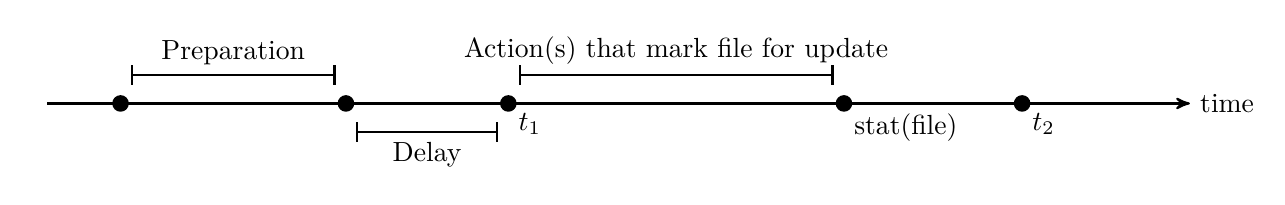
\begin{tikzpicture}[->,scale=1,>=stealth',thick,every text node part/.style={align=center}]


\node[] (ROOT) {};
\node[right=00.5cm of ROOT.east, anchor = west, text width=0.6cm] (PREP1) {};
\fill (PREP1) circle (3pt) node[above=0.1cm] {};
\node[above=0.1cm of PREP1.north, anchor = south] (PREP1ABOVE) {};

\node[right=2cm of PREP1.east, anchor = west, text width=0.6cm] (PREP2) {};
\fill (PREP2) circle (3pt) node[above=0.1cm] {};
\node[below=0.1cm of PREP2.south, anchor = north] (PREP2BELOW) {};
\node[above=0.1cm of PREP2.north, anchor = south] (PREP2ABOVE) {};

\node[right=1.5cm of PREP2.east, anchor = west, text width=0cm] (DELAY2) {};
\node[below=0.1cm of DELAY2.south, anchor = north] (FCLOSE_ARROW1) {};
\fill (DELAY2) circle (3pt) node[below right] {$t_{1}$};
% \node[below=-0.1cm of DELAY2.south, anchor = north] (FREAD_ARROW1) {};
% \node[below=0.8cm of DELAY2.south, anchor = west] (FREAD_ARROW2) {TB};
% \draw [->] (FREAD_ARROW2) -- node[above](){} (FREAD_ARROW1);
\node[above=0.1cm of DELAY2.north, anchor = south] (DELAY2ABOVE) {};


% \node[right=2cm of DELAY2.east, anchor = west, text width=0cm, inner sep=0, outer sep = 0] (ACTION) {};
% \fill (ACTION) circle (3pt) node[above=0.1cm] {action};
% 
\node[right=4cm of DELAY2.east, anchor = west, text width=0cm] (STAT) {};
\fill (STAT) circle (3pt) node[below right] {stat(file)};
% \node[below=-0.1cm of STAT.south, anchor = north] (STAT_ARROW1) {};
% \node[below=0.8cm of STAT.south, anchor = west] (STAT_ARROW2) {stat(file)};
% \draw [->] (STAT_ARROW2) -- node[above](){} (STAT_ARROW1);
\node[above=0.1cm of STAT.north, anchor = south] (STATABOVE) {};

\node[right=2cm of STAT.east, anchor = west, text width=0cm] (TA) {};
\fill (TA) circle (3pt) node[below right] {$t_{2}$};
% \node[below=-0.1cm of TA.south, anchor = north] (FREAD_ARROWTA1) {};
% \node[below=0.8cm of TA.south, anchor = west] (FREAD_ARROWTA2) {TA};
% \draw [->] (FREAD_ARROWTA2) -- node[above](){} (FREAD_ARROWTA1);

\node[right=2cm of TA.east, anchor = west, text width=0.6cm] (T) {time};
% \draw [-] (ROOT) -- node[above](Z1){} (PREP1);
% \draw [-] (PREP1) -- node[above](Z2){} (PREP2);
% \draw [-] (PREP2) -- node[above](Z3){} (DELAY2);
\draw [->] (ROOT) -- node[above](Z4){} (T);

\draw [|-|] (PREP1ABOVE) -- node[above](){Preparation} (PREP2ABOVE);
\draw [|-|] (PREP2BELOW) -- node[below](){Delay} (FCLOSE_ARROW1);
\draw [|-|] (DELAY2ABOVE) -- node[above](){Action(s) that mark file for update} (STATABOVE);

% \node[state, below left=0.5cm and 0.6cm of GRAP, \nodedisascolor, text width=3.6cm] (DISAS) {Disassembly\footnotemark: python (based on Capstone)};
% % \node[state, right=0.1cm of ASM.east, draw=none, anchor = west] (EQ) {=};
% % \node[state, right=0.8cm of DISAS.north east, anchor = north west, text width=4cm] (GRISO) {Graphes :};
% \node[state, right=4cm of DISAS.east, anchor = west, text width=3cm, minimum height=2.2cm, \nodedotcolor] (DOT) {DOT parser:\\ flex + bison (C)};
% \node[state, right = -0.05cm of DOT.north east, anchor = north west, text width=3cm, minimum height=2.2cm, \nodegtsicolor] (GTSI) {Graph matching:\\ C++};
% \node [fit={($(DOT.north west) + (-0, 0)$) ($(GTSI.south east) + (0, 0)$)}, draw, label=grap-match (binary)] (GRAPHES) {};
% \draw [->] (GRAP) -- node[above left]{import} (DISAS);
% \draw [->] (GRAP) -- node[above]{exec} (GRAPHES);
% 
% 
% \node[state, below=2.4cm of DISAS.west, anchor = west, text width=2.2cm] (EXE) {backspace.exe};
% \node[state, right=2cm of EXE.east, anchor = west, text width=2.2cm] (MDOT) {backspace.dot};
% \node[state, below right=0.8cm and 2cm of MDOT.east, anchor = north, text width=2cm] (PATTERN) {pattern.dot};
% \node[state, right=5cm of MDOT.east, anchor = west, text width=2cm] (MATCH) {match + extraction};
% 
% 
% \draw [->] (EXE) -- node[above right](EXEDOT){} (MDOT);
% \draw [->] (DISAS) -- (EXEDOT);
% 
% \coordinate [above=0.8cm of PATTERN.north] (INT);
% \draw [-] (MDOT) -- (INT);
% \draw [-] (PATTERN) -- (INT);
% \draw [->] (INT) -- node (DOTMATCH){} (MATCH);
% \draw [->] (GRAPHES) -- (DOTMATCH);

% \footnotemark
% \draw [->] (EXE) -- (MDOT);

% \draw [-] (GRAP) -- (DISAS) {Appel};
% \draw (PC) -- node[left=0.7cm]{Assemblage} (ASM);
% \draw [-] (TEXT) -- (PRINTF);
% \draw [-] (DATA) -- (HELLO);
% \draw (ASM) -- node[above=0.5cm]{Assemblage} (BIN);
\end{tikzpicture}
% \end{center}

% \end{preview} % VS
\end{document}
